\documentclass[11pt]{article}
% Packages
% ---
\usepackage{listings} % Source code formatting and highlighting 
\usepackage{fullpage}
\usepackage{color}
\usepackage{xcolor}
\usepackage{xparse}
\usepackage{graphicx}

% Title variables
% --- 
\author{ 
	Dylan Phelan \\ 
	Working With Corpora \\ 
	Professor Gregory Crane 
}
\title{Assignment 2}
\date{September 21, 2018}
 
% Definitions
% ---- 
% Colors
\definecolor{lightCyan}{HTML}{62929E}
\definecolor{khaki}{HTML}{C3B299}
\definecolor{orange}{HTML}{FFA552}
\definecolor{gray}{HTML}{A1A0AA}
\definecolor{olive}{HTML}{516D27}
% Envs
\newenvironment{solution}{
	\vspace{10px}\noindent\emph{Solution:}
}{
	\vspace{10px}
}
% Cmds
\newcommand{\codeword}[1]{
	\texttt{\textcolor{lightCyan}{#1}}
}
% Define our code blocks
\lstset{
	frame=tb,
	language=Python,
	aboveskip=2mm,
	belowskip=2mm,
	showstringspaces=false,
	columns=flexible,
	basicstyle={\small\ttfamily},
	numberstyle=\textcolor{khaki},
	keywordstyle=\textcolor{orange},
	commentstyle=\textcolor{gray},
	stringstyle=\textcolor{olive},
	breaklines=true,
	breakatwhitespace=true,
	tabsize=3
}

 
\begin{document}
\maketitle

\section*{Exercises for Chapter 2: Accessing Text Corpora and Lexical Resources}
\subsection*{Problem 1}

Create a variable \codeword{phrase} containing a list of words. Review the operations described in the previous chapter, including addition, multiplication, indexing, slicing, and sorting.

\begin{solution}
	
	We can start by defining a variable \codeword{phrase} and \emph{add} a bit more detail to it
	\begin{lstlisting}
		>>> phrase = ["This", "should", "satisfy", "question", "one's", "requirements"]
		>>> phrase = phrase + [',' 'I', 'hope', ]
		>>> phrase
        ['This', 'should', 'satisfy', 'question', "one's", 'requirements', ',I', 'hope', '!']
	\end{lstlisting}

    Maybe we want \emph{multiply} our enthusiasm 
	\begin{lstlisting}
		>>> enthusiasm_multiplier = ["!"]
		>>> enthusiasm_multiplier *= 5
		>>> enthusiasm_multiplier
		['!', '!', '!', '!', '!']
		>>> phrase += enthusiasm_multiplier
		>>> phrase
		['This', 'should', 'satisfy', 'question', "one's", 'requirements', ',I', 'hope', '!', '!', '!', '!', '!', '!']
	\end{lstlisting}

	Let's \emph{slice} out that uncertainty and infuse a bit of confidence into that phrase. You know who has confidence? \emph{Index}-fund traders... {\tiny a stretch, I know}
	\begin{lstlisting}
		>>> phrase[6:8]
		[',I', 'hope']
		>>> phrase = phrase[0:6] + phrase[8:]
		>>> phrase
		['This', 'should', 'satisfy', 'question', "one's", 'requirements', '!', '!', '!', '!', '!', '!']
		>>> phrase[1]
		'should'
		>>> phrase[1] = 'will'
		>>> phrase
		['This', 'will', 'satisfy', 'question', "one's", 'requirements', '!', '!', '!', '!', '!', '!']
		>>>
	\end{lstlisting}
	
	And I can't seem to \emph{sort} out a good pun for this last operation... so this meta-pun will have to do.
	\begin{lstlisting}
		>>> yoda_phrase = sorted(phrase)
		>>> yoda_phrase
		['!', '!', '!', '!', '!', '!', 'This', "one's", 'question', 'requirements', 'satisfy', 'will']
	\end{lstlisting}
	
\end{solution} 


\subsection*{Problem 2}
Use the corpus module to explore austen-persuasion.txt. How many word tokens does this book have? How many word types?

\begin{solution}
	
	98171 word tokens, and 6132 word types, as determined by the following code:
	
	\begin{lstlisting}
		>>> from nltk.corpus import gutenberg
		>>> gutenberg.words('austen-persuasion.txt')
		['[', 'Persuasion', 'by', 'Jane', 'Austen', '1818', ...]
		>>> words = len(gutenberg.words('austen-persuasion.txt'))
		>>> words
		98171
		>>> word_types = set(gutenberg.words('austen-persuasion.txt'))
		>>> len(word_types)
		6132
	\end{lstlisting}
	
\end{solution}  


\subsection*{Problem 3}
Use the Brown corpus reader nltk.corpus.brown.words() or the Web text corpus reader nltk.corpus.webtext.words() to access some sample text in two different genres.

\begin{solution}
	
	Let's see what terms lie at the interesection of hobbies and sci\_fi, looking only at the first 200 and only at terms that are longer than five characters
	\begin{lstlisting}
		>>> from nltk.corpus import brown
		>>> brown.categories()
		['adventure', 'belles_lettres', 'editorial', 'fiction', 'government', 'hobbies', 'humor', 'learned', 'lore', 'mystery', 'news', 'religion', 'reviews', 'romance', 'science_fiction']
		>>> hobbies_words = brown.words(categories="hobbies")
		>>> hobbies_words
		['Too', 'often', 'a', 'beginning', 'bodybuilder', ...]
		>>> sci_fi_words = brown.words(categories="science_fiction")
		>>> sci_fi_words
		['Now', 'that', 'he', 'knew', 'himself', 'to', 'be', ...]
		>>> sci_fi_hobby_words = set(hobbies_words).intersection(set(sci_fi_words))
		>>> fdistf_sci_fi_hobbies_terms = nltk.FreqDist(w.lower() for w in sci_fi_hobby_words)
		>>> fdist_sci_fi_hobbies_terms = nltk.FreqDist(w.lower() for w in sci_fi_hobby_words)
		>>> [word for (word, freq) in fdist_sci_fi_hobbies_terms.most_common(200) if len(word) > 5]
		['school', 'according', 'neither', 'though', 'without', 'sometimes', 'actually', "you've", "there's", "that's", 'western', 'system', 'another', 'nevertheless', 'therefore', 'nobody', 'almost', 'before', 'through', 'perhaps', 'having', 'animals', 'nations', 'southern', 'behind', 'although', 'between', 'instead', 'service', 'states', 'however', 'nothing', 'second', 'function', "you're", 'selective', 'lifted', 'children', 'species', 'special', 'electronic', 'knotty', 'nerves', 'fertile', 'stayed', 'condition', 'seeing', 'identical', "they'll", 'century', 'immediate', 'wanted', 'estimate', 'content', 'vacuum', 'lessons', 'valuable', 'equipment', 'distinguished', 'gently', 'commonplace', 'shining', 'contained']
	\end{lstlisting}
	
\end{solution}  


\subsection*{Problem 4}
Read in the texts of the State of the Union addresses, using the state\_union corpus reader. Count occurrences of men, women, and people in each document. What has happened to the usage of these words over time?

\begin{solution}
	
	Based on the figure below, we can determine a few insights: 
	\begin{enumerate}
		
		\item The term 'women' is consistently less popular than the term 'men' until the 1970's, after which time the two are much more consistent in frequency.
		
		\item The term 'people' has historically been a more popular term than 'men' or 'women'.
		
		\item The term 'people' had a major spike in popularity the mid 90's.
		
		\item The use of the term 'people' looks like it has been on the decline in the last 10 years of recorded data, whereas the terms 'men' and 'women' are increasing in popularity in that same period.
	\end{enumerate}
	\hspace*{-50pt}
	% Link to the state of the union conditional frequency figure
	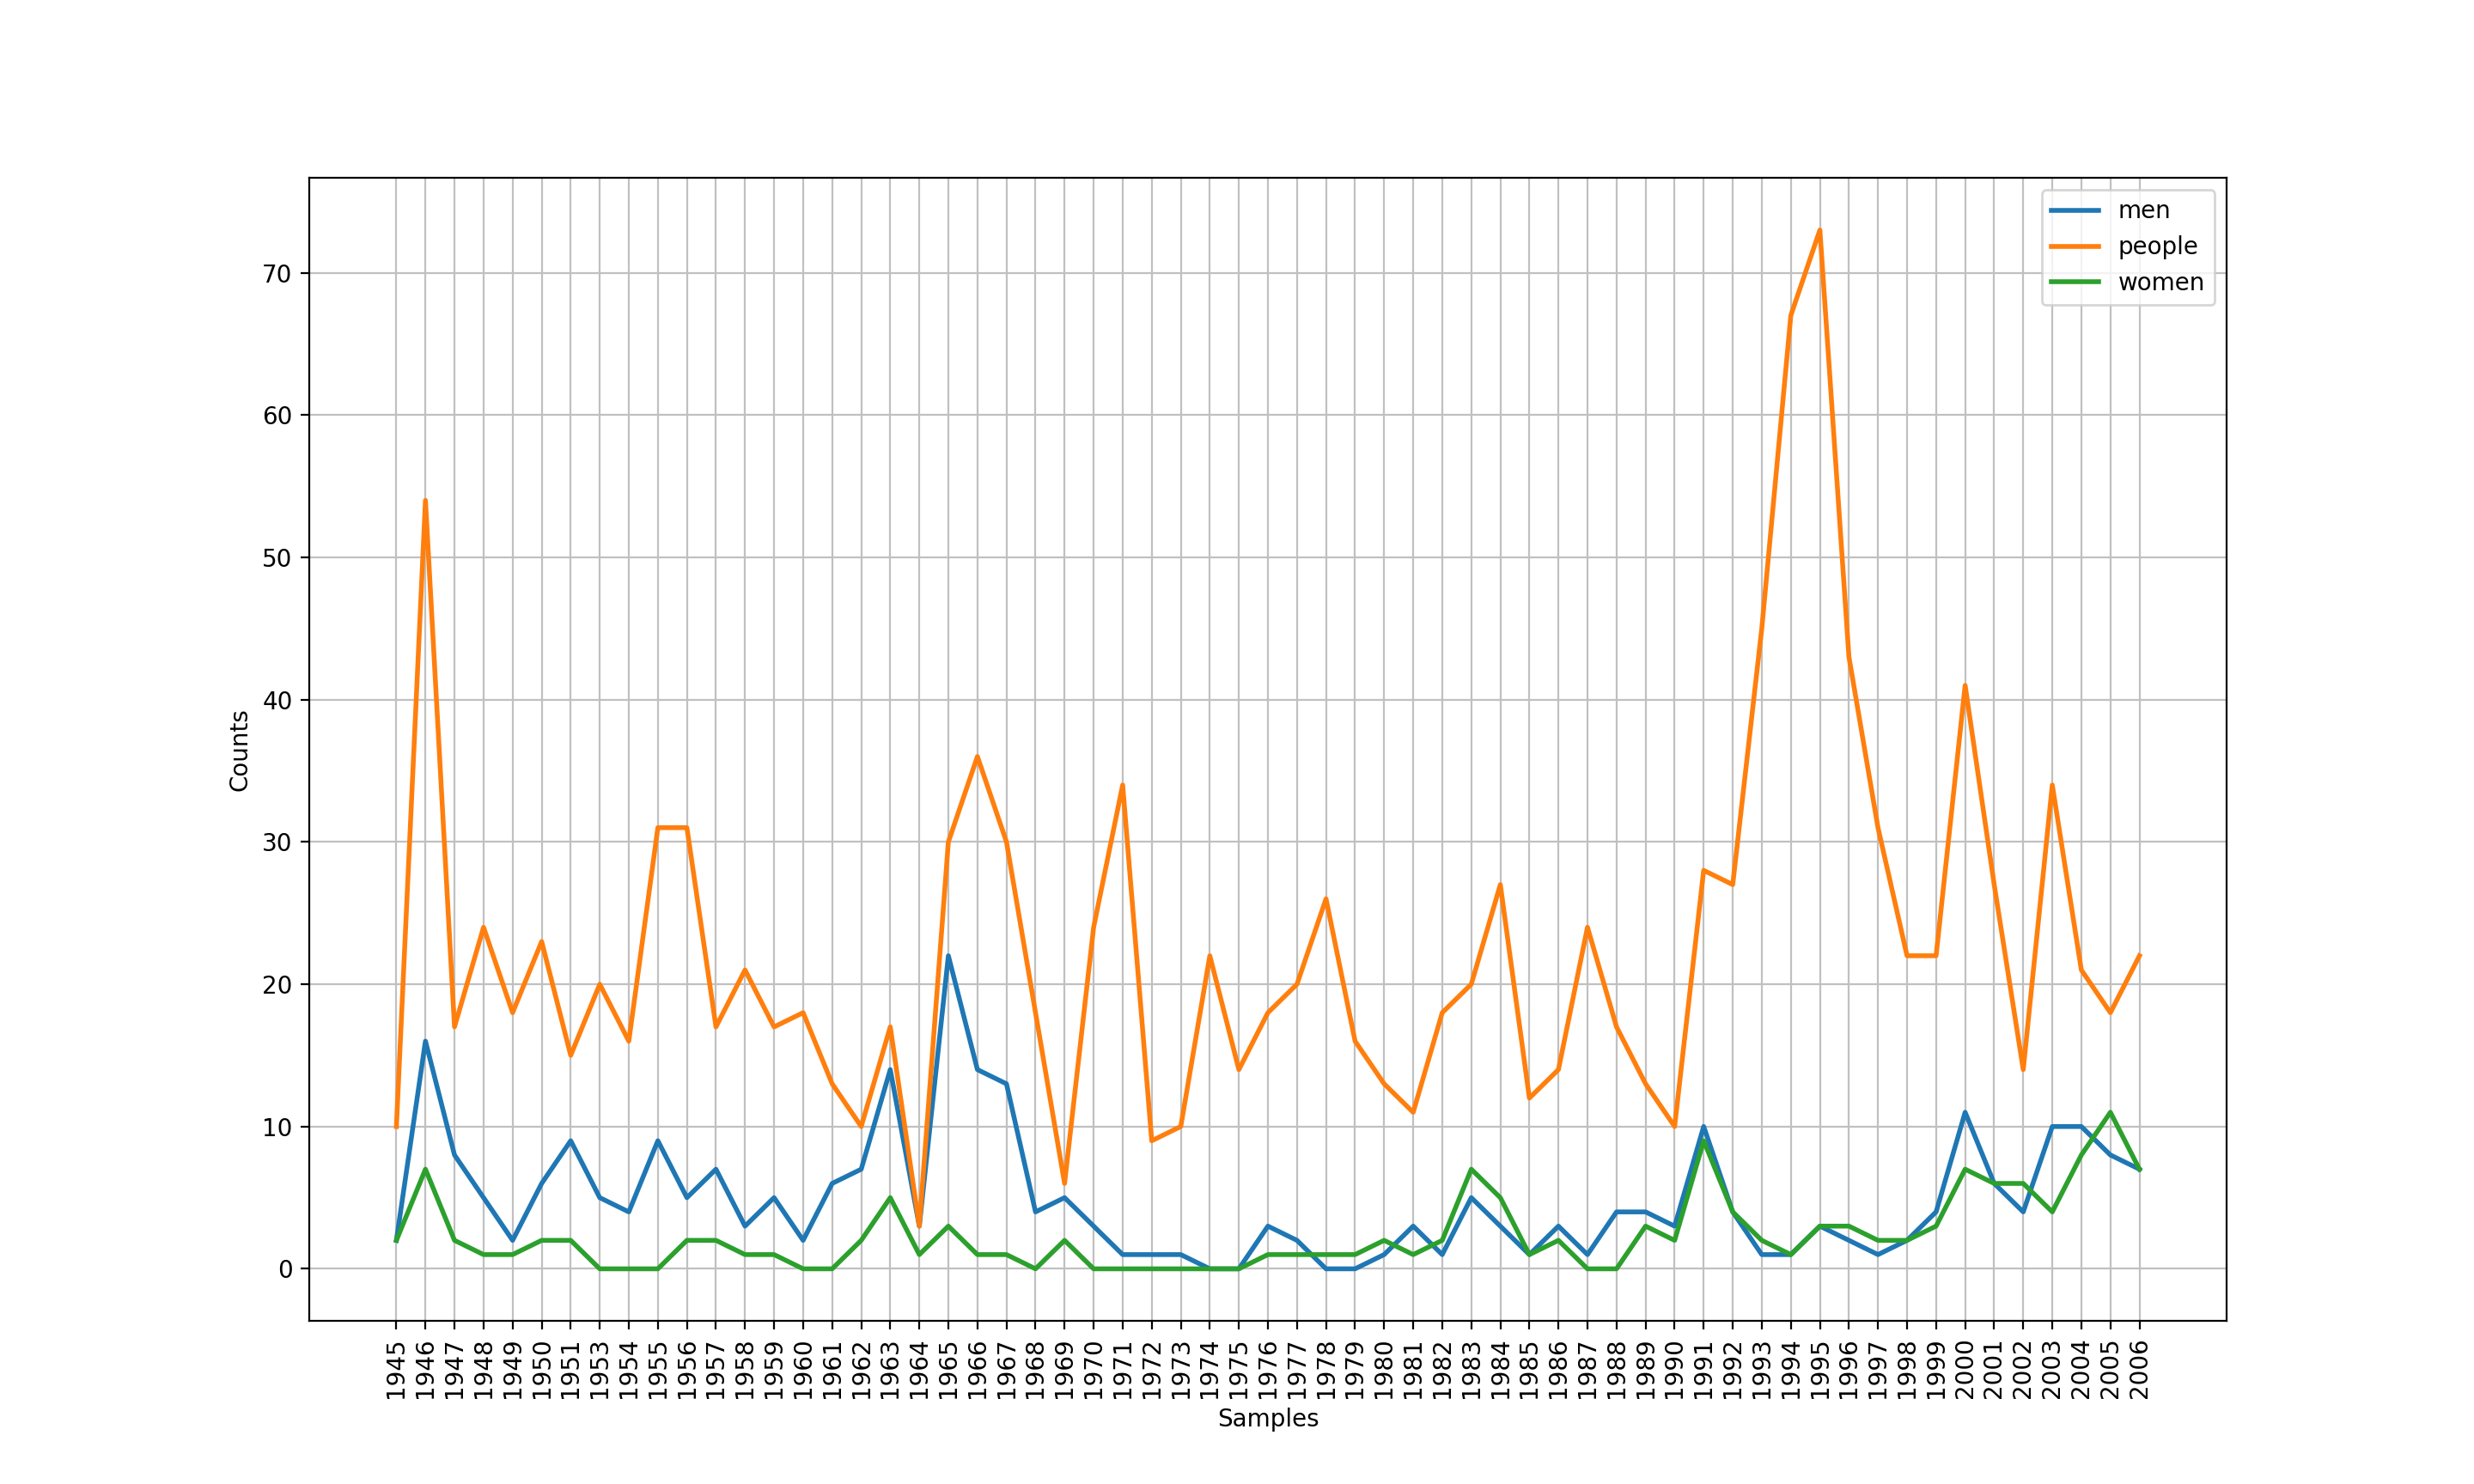
\includegraphics[width=550pt]{state_of_the_union_comp_men_people_women.png}
	Generated with the following code:
	\begin{lstlisting}
		>>> from nltk.corpus import state_union
		>>> cfd = nltk.ConditionalFreqDist(
		...     (target, fileid[:4])
		...     for fileid in state_union.fileids()
		...     for w in state_union.words(fileid)
		...     for target in ['men', 'women', 'people']
		...     if w.lower().startswith(target)
		... )
		>>> cfd.plot()
	\end{lstlisting}
	
\end{solution}  


\subsection*{Problem 5}
Investigate the holonym-meronym relations for some nouns. Remember that there are three kinds of holonym-meronym relation, so you need to use: member\_meronyms(), part\_meronyms(),  substance\_meronyms(), member\_holonyms(), part\_holonyms(), and substance\_holonyms().

\begin{solution}
	
	Originally I was trying individual terms that I thought could have various types of meronyms and holonyms, which was painfully fruitless. To investigate the problem more deeply, I wrote a small script that could print out various terms with holonyms and meronyms from Moby Dick, as provided by the \codeword{nltk.book} module: 
	
	\begin{lstlisting}
		>>> from nltk.book import *
		>>> from nltk.corpus import wordnet as wn
		>>> vocab_1 = list(set(w.lower() for w in text1 if len(w) >= 4))
		>>> for w in vocab_1[:600]:
		...     avail_synsets = wn.synsets(w)
		...     if len(avail_synsets) > 0:
		...         # For all the synsets, look for holobyms and meronyms
		...         for synset in avail_synsets:
		...             member_m = synset.member_meronyms()
		...             part_m = synset.part_meronyms()
		...             substance_m = synset.substance_meronyms()
		...             member_h = synset.member_holonyms()
		...             part_h = synset.part_holonyms()
		...             substance_h = synset.substance_holonyms()
		...             # If we have any valid holonyms or meronyms, print them out for viewing
		...             if (member_m or part_m or substance_m or member_m or part_m or substance_m):
		...                 print('\n\nSynset: ', synset)
		...                 if (member_m or part_m or substance_m):
		...                     print("--- meronyms")
		...                     if len(member_m) > 0: print("member_m: ", member_m)
		...                     if len(part_m) > 0: print("part_m: ", part_m)
		...                     if len(substance_m) > 0: print("substance_m: ", substance_m)
		...                 if (member_h or part_h or substance_h):
		...                     print("--- holonymss")
		...                     if len(member_h) > 0: print("member_h: ", member_h)
		...                     if len(part_h) > 0: print("part_h: ", part_h)
		...                     if len(substance_h) > 0: print("substance_h: ", substance_h)
	\end{lstlisting}
	
	Which provided many examples of these different types of holonyms and meronyms. Too many to include, but I've highlighted a few I thought were interesting that also cover all 6 cases:
	\begin{lstlisting}
		
		Synset:  Synset('flock.n.05')
		--- meronyms
		member_m: A constituent member of the above Synset term:  [Synset('sheep.n.01')]
		
		
		Synset:  Synset('shirt.n.01')
		--- meronyms
		part_m: Part of the above Synset term:  [Synset('dickey.n.02'), Synset('shirt_button.n.01'), Synset('shirtfront.n.01'), Synset('shirtsleeve.n.01'), Synset('shirttail.n.02')]
		substance_m: The substance of the above synset term:  [Synset('shirting.n.01')]
		
		
		Synset:  Synset('pine.n.01')
		--- meronyms
		part_m: Part of the above Synset term:  [Synset('pinecone.n.01')]
		substance_m: The substance of the above synset term:  [Synset('pine.n.02')]
		--- holonymss
		member_h: The above Synset term is a member of:  [Synset('pinus.n.01')]
		
		
		Synset:  Synset('sea.n.01')
		--- meronyms
		part_m: Part of the above Synset term:  [Synset('bay.n.01'), Synset('gulf.n.01'), Synset('inlet.n.01')]
		--- holonymss
		part_h: The above Synset term is a part of:  [Synset('hydrosphere.n.01')]
		
		Synset:  Synset('wine.n.01')
		--- holonymss
		substance_h: The above Synset term is made of:  [Synset('grape.n.01'), Synset('negus.n.01')]
		
	\end{lstlisting}
\end{solution}  


\subsection*{Problem 9}
Pick a pair of texts and study the differences between them, in terms of vocabulary, vocabulary richness, genre, etc. Can you find pairs of words which have quite different meanings across the two texts, such as monstrous in Moby Dick and in Sense and Sensibility?

\begin{solution}
	Looking at Whitman's "Leaves of Grass" and the Melville's "Moby Dick", we could highlight the following features and key differences: 
	\begin{enumerate}
		
		\item Whitman - Vocab:  12324  Richness:  0.07956973973902881
		
		\item Melville - Vocab:  16948  Richness:  0.06497992860949547
		
		\item The collocations in "Leaves of Grass" highlight themes of nature, time, growth, and cycles of change, whereas the collocations in "Moby Dick" highlight the books nautical nature, characters and the central role of whales in the book.
		
		\item Using the \codeword{text.similar(term)} function on some common adjectives in the english language, we don't such a difference in usage as distinct in the example above; but we do see a difference in the things being described by the adjectives, Whitman referring more often to the Earth as soil and Terra and sky, whereas Melville more often than not will be describing the sea and the creatures within. Below I've provided example code for the terms 'main', 'dark', and 'cold'.
	
	\end{enumerate}
	
	\begin{lstlisting}
		>>> whit = nltk.Text(nltk.corpus.gutenberg.words('whitman-leaves.txt'))
		>>> moby = nltk.Text(nltk.corpus.gutenberg.words('melville-moby_dick.txt'))
		>>> def vocab_len(txt):
		...     return len(set(w.lower() for w in txt if w.isalpha()))
		...
		>>> def vocab_richness(txt):
		...     return vocab_len(txt) / len(txt)
		...
		>>> print("Vocab: ", vocab_len(whit), " Richness: ", vocab_richness(whit))
		Vocab:  12324  Richness:  0.07956973973902881
		>>> print("Vocab: ", vocab_len(moby), " Richness: ", vocab_richness(moby))
		Vocab:  16948  Richness:  0.06497992860949547
		>>> whit.collocations()
		young men; open air; Walt Whitman; young man; New World; every one;
		every thing; whole earth; Thou knowest; thousand years; Old Age; old
		man; shapes arise; little child; old age; centuries hence; thousand
		miles; became part; every day; comes back
		>>> moby.collocations()
		Sperm Whale; Moby Dick; White Whale; old man; Captain Ahab; sperm
		whale; Right Whale; Captain Peleg; New Bedford; Cape Horn; cried Ahab;
		years ago; lower jaw; never mind; Father Mapple; cried Stubb; chief
		mate; white whale; ivory leg; one hand
		>>>
		>>> whit.similar('cold')
		day best by body long the earth trees here now them action me perfect
		good sea spreading white land sky
		>>> moby.similar('cold')
		green first heart body world hand whale word english whales case eye
		eyes lord day sea mouth land days foam
		>>>
		>>> whit.similar('dark')
		night earth rest dead soul woman past air ground grass war sea day sky
		stars woods globe water streets one
		>>> moby.similar('dark')
		deep sea other head captain air pacific wide wild fine light by the
		body all world whale fish word that
		>>>
		>>> whit.similar('main')
		last true mountain grass soul body in other earth trees waves first
		book top far male modern man poets old
		>>> moby.similar('main')
		world ship body whale whales case sea life seas water way head voyage
		captain boats fire matter line time soul
	
	\end{lstlisting}
	
	
\end{solution}  


\subsection*{Problem 23}
Let f(w) be the frequency of a word w in free text. Suppose that all the words of a text are ranked according to their frequency, with the most frequent word first. Zipf's law states that the frequency of a word type is inversely proportional to its rank (i.e. f × r = k, for some constant k). For example, the 50th most common word type should occur three times as frequently as the 150th most common word type.
Write a function to process a large text and plot word frequency against word rank using pylab.plot. Do you confirm Zipf's law? (Hint: it helps to use a logarithmic scale). What is going on at the extreme ends of the plotted line?
\begin{enumerate}
	\item Write a function to process a large text and plot word frequency against word rank using pylab.plot. Do you confirm Zipf's law? (Hint: it helps to use a logarithmic scale). What is going on at the extreme ends of the plotted line?
	\item Generate random text, e.g., using random.choice("abcdefg "), taking care to include the space character. You will need to import random first. Use the string concatenation operator to accumulate characters into a (very) long string. Then tokenize this string, and generate the Zipf plot as before, and compare the two plots. What do you make of Zipf's Law in the light of this?
\end{enumerate}

\begin{solution}
	Solution goes here
\end{solution}  


\section*{Research Publication of Interest} Identify a recent research publication that interests you. Write a very short summary and explain why you found it interesting. Be prepared to discuss this in class next week. Suggested publications include (but are by no means limited to): 

\begin{enumerate}
	\item Digital Humanities Quarterly (DHQ): http://www.digitalhumanities.org/dhq/ 
	
	\item The Human Language Technology Conference (HLT): https://aclanthology.coli.uni-saarland.de/venues/hlt
	
	\item Any publication that catches your eye in the Association for Computational Linguistics Anthology: https://aclanthology.coli.uni-saarland.de/ 
	
	\item Anything that you know of and think would suit the content of the class.
	
	
\end{enumerate}


\end{document}